\chapter{Lo studio dei mesoni composti da quark charm }

\section{Il Modello Standard}
Per quanto riguarda la fisica delle particelle, il modello che attualmente ne descrive i fondamenti è il \textit{Modello Standard}. In questo modello le particelle fondamentali sono divise tra fermioni e bosoni. 

La figura \ref{fig:ModelloStandard} rappresenta uno schema delle particelle previste dal Modello Standard.
    \begin{figure}[htbp]
        \centering
        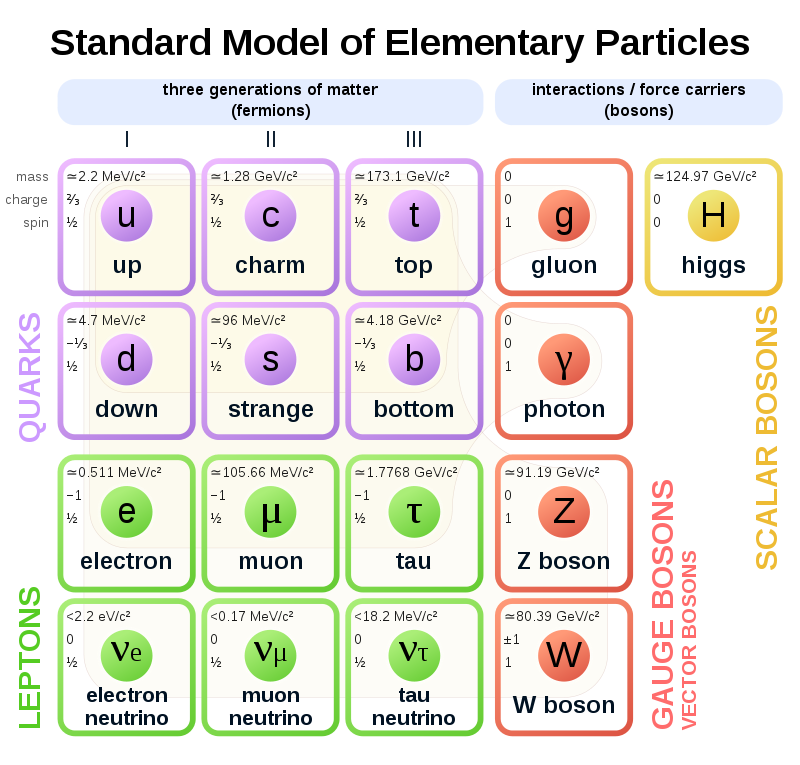
\includegraphics[width=0.65\linewidth]{introParticelle/ModelloStandard.png}
        \caption{Rappresentazione del Modello Standard}
        \label{fig:ModelloStandard}
    \end{figure}
Nella parte sinistra della figura si trovano i \textit{fermioni} divisi tra quark e leptoni. I fermioni sono divisi in tre generazioni ordinate in base a valori di massa crescente. I quark sono contraddistinti dal sapore (up, down, charm, strange, top e bottom) e si combinano per formare barioni (3 quark) o mesoni (coppie di un quark e un anti-quark). Nella parte destra della figura \ref{fig:ModelloStandard} si trovano i \textit{bosoni} che comprendono i bosoni di Gauge, che sono i mediatori delle forze fondamentali previste dal Modello Standard, e il bosone di Higgs, che è l'unico bosone scalare (con spin 0) identificato per la prima volta nel 2012 al Cern. In questa tesi ci si occuper\`a in particolare dei mesoni contenenti un quark charm, la cui importanza e' descritta nel seguito.
 
\section{I mesoni con charm nello studio del QGP}
Il \textit{Plasma di Quark e Gluoni} (QGP) è uno stato della materia in cui i quark e i gluoni non sono confinati negli adroni dalla forza nucleare forte. Gli adroni formati da quark pesanti (come il charm) sono un buono strumento per studiare il QGP formatosi dalla collisione di ioni pesanti. Infatti, il quark charm ha un tempo di formazione pari a $\frac{\hbar}{2m_qc^2} \leq 0.1 \ \mathrm{fm/c} \simeq 0.3 10^{-24}$ s che \`e minore del tempo di formazione del QGP $\simeq (0.3 - 1.5) \ \mathrm{fm/c} \simeq 10^{-24} - 0.5 \ 10^{-23}$ s. Quindi i quark charm, prodotti prima della formazione del QGP, attraversano il QGP stesso e interagiscono con i suoi componenti permettendo di avere informazioni sulle propriet\`a del QGP stesso. Inoltre, i quark pesanti preservano la loro identit\`a mentre attraversano il QGP e infine adronizzano formando adroni che possono essere osservati dai rivelatori di ALICE. I mesoni D, che verranno presi in considerazione in questa tesi, sono formati da un quark charm e un quark pi\`u leggero e costituiscono pertanto delle buone osservabili per lo studio del QGP. 

È di fondamentale importanza studiare la produzione di adroni composti da quark pesanti non solo in collsioni di ioni, ma anche in collisioni protone-protone in cui non ci si aspetta la formazione del QGP.
Infatti soltanto dal paragone della produzione nei due sistemi \`e possibile ricavare informazioni sull'interazione dei quark charm con il QGP. 
\\Inoltre la misura di produzione di mesoni D in collisioni protone-protone rappresenta un'ottima verifica per la Cromo-Dinamica Quantistica (QCD), teoria che permette di calcolare teoricamente la produzione di quark charm e la successiva adronizzazione.

\section{Il mesone $D^{*+}$} \label{mesoneD}
In questa tesi si \`e considerato in particolare il mesone $D^{*+}$, che \`e formato da un quark charm $c$ e un anti-quark down $\overline{d}$ ed ha momento angolare totale 1, e la sua antiparticella $D^{*-}$. Il mesone $D^{*+}$ ha una massa di ($2010.26 \pm 0.05$) MeV/$c^2$ e vita media $ \tau = (7.89 \pm 0.11) {10^{-21}}$~ s~\cite{PDG}. Il decadimento studiato in questa tesi \`e il decadimento forte:
    \begin{equation}
         D^{*+} \rightarrow D^0 + \pi^+ 
    \end{equation}
    che ha un branching ratio BR = $67.7 \%$. 
    Il mesone $D^0$ ha massa $ (1864.83 \pm 0.05)$~ MeV/$c^2$, decade con decadimento debole $D^0 \rightarrow K^- \pi^+$ con un BR = $3.89 \%$ ed ha una vita media di $(410.1 \pm 1.5 ) 10^{-15}$~s~\cite{PDG}.
\\Nel caso in cui la $D^{*+}$ decada da ferma, il pione ha un impulso di soli $39$ MeV/c e veine indicato come $\pi_{soft}$. \\Il Q-valore del decadimento \`e:
    \begin{equation}
        Q = m_{D^{*+}} - (m_{D^{0}} + m_{\pi_{soft}}) = 5.93 \ \mathrm{MeV/c^2}
    \end{equation}

La figura \ref{fig:decadimentoD} rappresenta la topologia del decadimento del mesone $D^{*+}$. Il punto di decadimento della $D^{*+}$ \`e indistinguibile dal vertice primario, ovvero il punto in cui avviene la collisione dei fasci di protoni, a causa delle distanze che caratterizzano il decadimento forte. Il pione $\pi_{soft}$ emesso dal decadimento del mesone $D^{*+}$ viene direttamente rivelato dai rivelatori di ALICE. Il punto di decadimento del mesone $D^0$ (che decade con decadimento debole) \`e, invece, separato dal vertice primario di $c\tau = 122.9 \ \mu m $, dove $c$ \`e la velocit\`a della luce nel vuoto e $\tau$ la vita media del mesone $D^0$. Il punto di decadimento del mesone $D^0$ viene chiamato vertice secondario (SV).
 
    \begin{figure}[htbp]
        \centering
        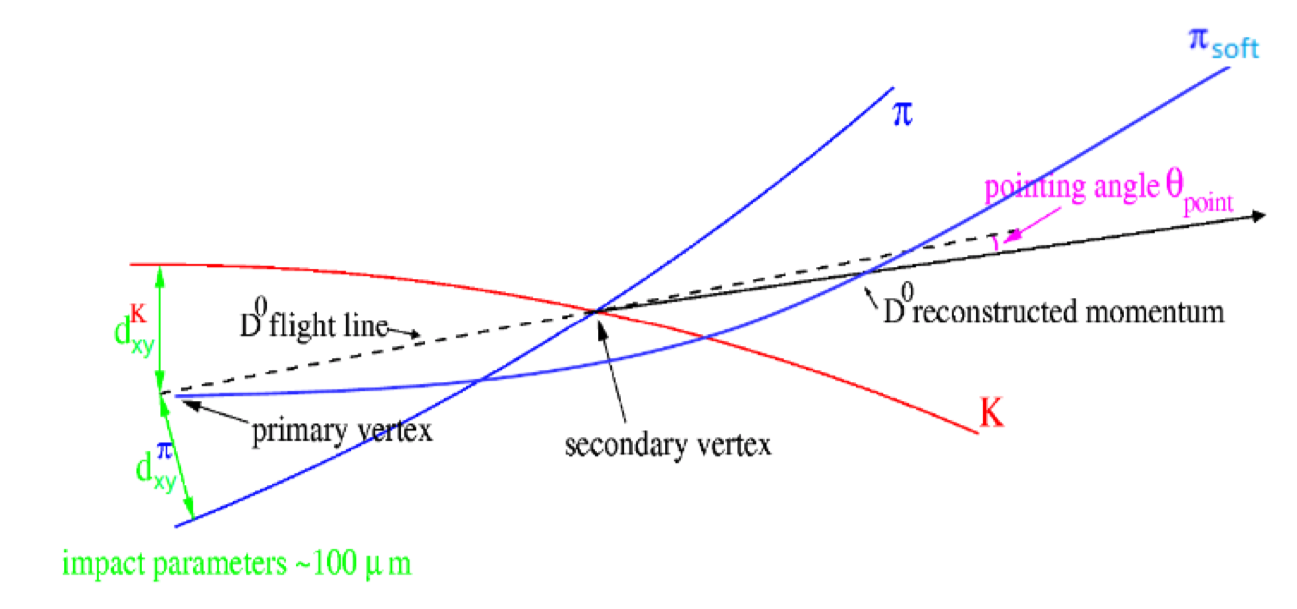
\includegraphics[width=0.9\linewidth]{introParticelle/DecadimentoDStar.png}
        \caption{Topologia del decadimento del mesone $D^{*+}$ nel canale $D^{*+} \rightarrow D^0 \pi^+$ e successivo decadimento $D^0 \rightarrow K^- \pi^+$. Il vertice di decadimento del mesone $D^{*+}$ \`e indistinguibile dal vertice primario a causa delle distanze caratteristiche dei decadimenti forti}
        \label{fig:decadimentoD}
    \end{figure}
    
Per identificare il mesone $D^{*+}$, inizialmente, si ricostruiscono le candidate $D^0$ considerando tutte le possibili combinazioni di due tracce di segno opposto. Successivamente le candidate $D^0$ cos\`i ricostruite vengono combinate con la traccia di un candidato pione. Per ridurre il fondo combinatoriale costituito dalle coppie $\pi^+ \ K^-$ che non vengono dal decadimento di un mesone $D^0$, vengono applicate delle selezioni sulle variabili topologiche.
\\Tali variabili topologiche sono riportate in figura \ref{fig:decadimentoD} e sono:
    \begin{itemize}
        \item la lunghezza di decadimento della $D^0$, ovvero la distanza tra il vertice primario e secondario;
        \item i parametri d'impatto del kaone e del pione (in figura \ref{fig:decadimentoD} indicati come ${d^K}_{XY}$ e ${d^\pi}_{XY}$ rispettivamente per kaone e pione), che sono la distanza minima tra la traiettoria di kaone o pione e il vertice primario;
        \item l'angolo di puntamento, indicato come $\theta_{point}$, che \`e l'angolo tra la retta congiungente il PV e il SV e la direzione del vettore impulso trasverso ($p_T$) della candidata $D^{0}$ ricostruita;
        \item l'angolo di decadimento, che \`e l'angolo tra il vettore impulso del mesone $D^0$ e il vettore impulso del $\pi^+$ nel sistema di riferimento della candidata $D^0$ ricostruita;
        \item la distanza di minimo approccio (DCA), ovvero la distanza minima tra le traiettorie del $K^-$ e del $\pi^+$ nel piano perpendicolare alla direzione del fascio.
    \end{itemize}{}

In aggiunta alla selezione sulle variabili topologiche, viene anche utilizzata l'identificazione di particelle con TPC e TOF per identificare il pione e il kaone derivanti dal decadimento del mesone $D^0$.
\\Nell'analisi standard di ALICE le selezioni sulle variabili topologiche indicate sopra vengono ottimizzate con una procedura manuale per massimizzare la quantit\`a di segnale rispetto al fondo combinatoriale. Nel lavoro presentato in questa tesi, l'analisi multivariata implementata nell'algoritmo del Boosted Decision Tree combina le variabili topologiche creando un'unica variabile discriminatoria finale.
\\Per determinare il numero di candidate $D^{*+}$ ricostruite  si utilizza un'analisi in massa invariante, quest'ultima \`e definita come: 
    \begin{equation}
        M = {E^2}_{TOT} - {p^2}_{TOT}
    \end{equation}
dove $E_{TOT}$ \`e l'energia totale di tutte le particelle del sistema considerato e $p_{TOT}$ \`e l'impulso totale. 
\\Nel caso della $D^0$ la massa invariante del doppietto pione-kaone \`e data da:  
    \begin{equation}
        M(K^- \pi^+) = ({E_{\pi^+}+E_{K^-}})^2 - ({p_{\pi^+}+p_{K^-}})^2
    \end{equation}
dove $E_{\pi^+}$ e $E_{K^-}$ sono le energie del pione e del kaone, $p_{\pi^+}$ e $p_{K^-}$ sono i rispettivi impulsi.
\\La massa invariante della candidata $D^{*+}$ \`e data da:
    \begin{equation}
        M(K^- \pi^+ \pi_{soft}) = ({E_{\pi^+}+E_{K^-}+E_{\pi_{soft}}})^2 - ({p_{\pi^+}+p_{K^-}+p_{\pi_{soft}}})^2
    \end{equation}
Dove $E_{\pi_{soft}}$ \`e l'energia del $\pi_{soft}$ e $p_{\pi_{soft}}$ \`e l'impulso del $\pi_{soft}$.
\\Il segnale relativo al mesone $D^{*+}$ si studia preferibilmente usando la variabile $\Delta M$
  \begin{equation}
       \Delta M = M (K^- \pi^+ \pi^+) - M(K^- \pi^+)
    \end{equation}
    
dove $ M (K^- \pi^+ \pi^+)$ \`e la massa invariante ricostruita della candidata $D^{*+}$ e $ M(K^- \pi^+)$ la massa invariante ricostruita della candidata $D^{0}$. La distribuzione della variabile $\Delta M$ mostra un picco al valore di circa $145$~ MeV/c. Si considera preferibilmente la distribuzione di $\Delta M$ in quanto nella sottrazione l'incertezza sull'impulso del kaone e del pione si cancellano e la larghezza del picco \`e determinata solo dalla risoluzione sull'impulso del $\pi_{soft}$. La figura \ref{fig:distribuzione_massa} mostra un esempio della distribuzione della differenza di massa invariante $\Delta M$ per candidate $D^{*+}$ con un impulso trasverso $p_T$ [3,4] GeV/c selezionate con l'analisi multivariata, come verr\`a spiegato nel capitolo \ref{applicazione}. A destra del picco di segnale \`e visibile il fondo combinatoriale. Su questo grafico si far\`a poi un fit sia del picco di segnale, sia del fondo per ottenere la quantit\`a di $D^{*+}$ selezionata. 

    \begin{figure}[htbp]
        \centering
        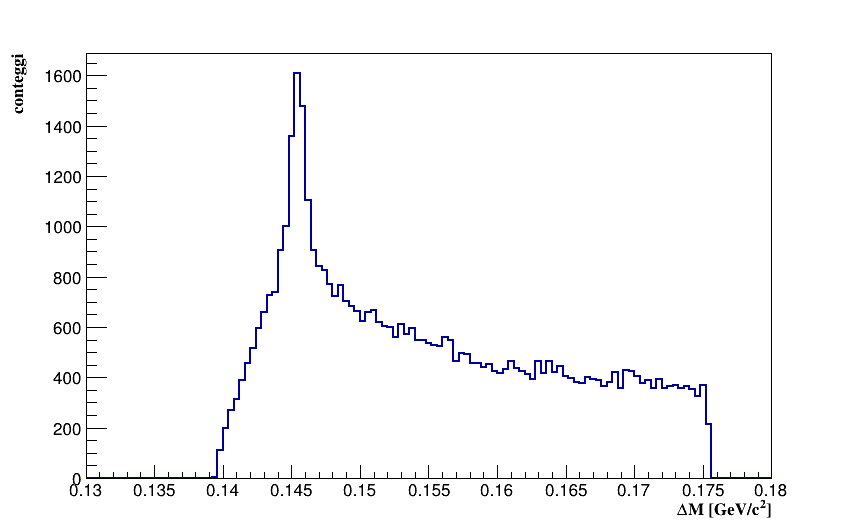
\includegraphics[width=0.8\linewidth]{AnalisiDati/diffDstarD0_3_4BDT.png}
        \caption{Distribuzione di massa invariante $\Delta M = M (K^- \pi^+ \pi^+) - M(K^- \pi^+)$ del campione di dati di ALICE nell'intervallo di impulso trasverso $p_T$ [3,4] GeV/c dopo l'applicazione dell'algoritmo BDT.}
        \label{fig:distribuzione_massa}
    \end{figure}



